\documentclass[12pt,a4paper]{scrartcl}
\usepackage[utf8]{inputenc}
\usepackage{amsmath}
\usepackage{amsfonts}
\usepackage{amssymb}
\usepackage{graphicx}

\usepackage[bottom = 1in, left = 0.5in, right = 0.5in, top = 1in]{geometry}

\usepackage[english]{babel}
\usepackage[autostyle]{csquotes}
% \usepackage{mathptmx}
\usepackage{bm}
\usepackage{caption}
\usepackage{float}
% Mark continued floats as a, b, ...
\renewcommand\theContinuedFloat{\roman{ContinuedFloat}}

\usepackage[labelfont=bf]{caption}

\usepackage[default, scale=0.95]{opensans} %% Alternatively
%% use the option 'defaultsans' instead of 'default' to replace the
%% sans serif font only.
\usepackage[T1]{fontenc}

\addto\captionsenglish{\renewcommand{\figurename}{Supplementary Fig.}}
\addto\captionsenglish{\renewcommand{\tablename}{Supplementary Table}}

\title{Supplementary materials}
\date{}

\begin{document}
\maketitle

\section*{Supplementary section 1}
\subsection*{Regions and ecosystems classification}

\begin{figure}[H]
	\centering
	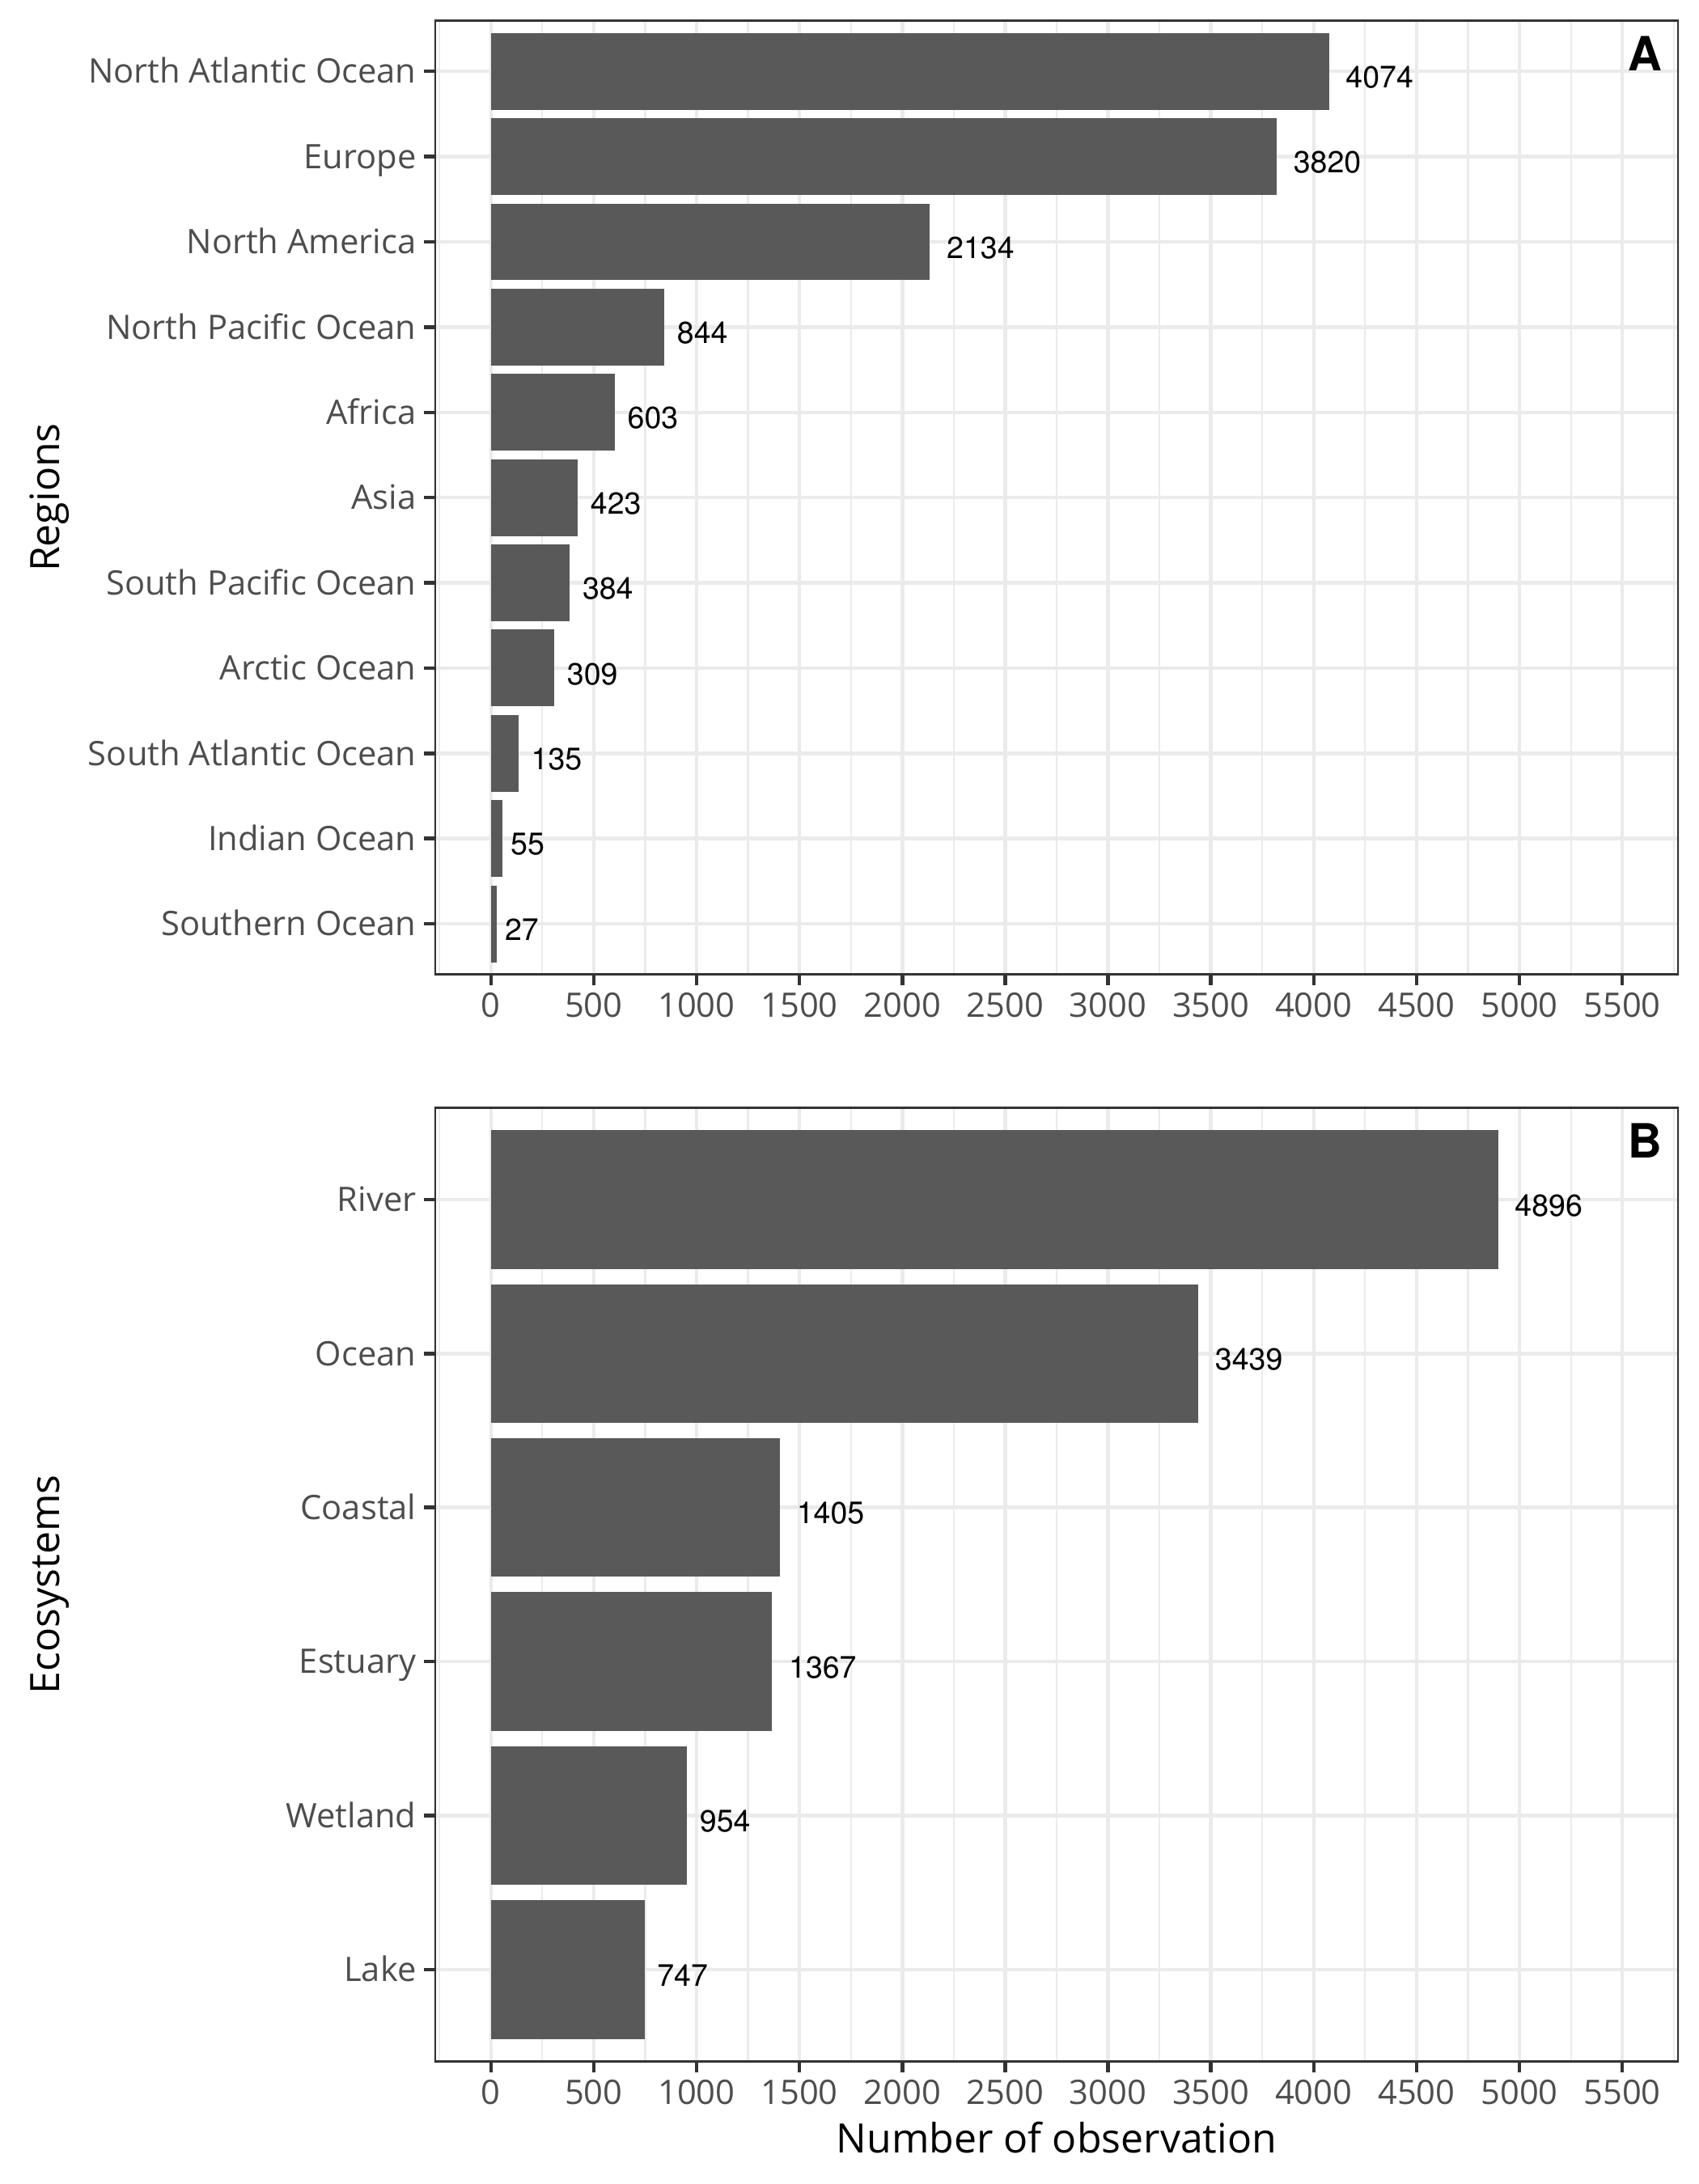
\includegraphics[scale = 1]{../../graphs/appendix1}
	\caption{Barplot showing the number of unique observations for (\textbf{A}) principal regions and (\textbf{B}) ecosystems.}
\end{figure}

\clearpage
\newpage

\section*{Supplementary section 2}
\subsection*{Estimation of \boldmath{$a_{\text{CDOM}}(350)$} from other wavelengths}

In the literature data, we found that a wide range of different wavelengths (between 250 and 490 nm) were used as reference wavelength to report absorption coefficients of CDOM (Supplementary Table 1). To make absorption coefficients comparable among studies, an interpolation procedure was used to estimate $a_{\text{CDOM}}(350)$ independently of the wavelength reported in each study. Between 250 and 350 nm, determination coefficients ($R^2$) gradually increased from 0.987 to 1 (Fig.~\ref{first}--A). After 350 nm, $R^2$ decreased rapidly to reach 0.86 at 500 nm. Between 250 and 500 nm, the regression slopes increased almost exponentially (0.28--6.99, Fig.~\ref{first}--B) whereas the intercepts increased more or less linearly between -1.4 and 1.5 m$^{-1}$ across the spectral range (Fig.~\ref{first}--C). Perfect fit at 350 nm is identified using vertical dashed lines where $R^2$ = 1, slope = 1 and intercept = 0. Note that the 95\% confidence interval of the estimated slope values is hardly distinguishable which emphasizes the robustness of the generated models (shaded area in Fig.~\ref{first}--B). Regression coefficients used to estimate $a_{\text{CDOM}}(350)$ in this study are presented in Supplementary Table 1. Absorption coefficients measured at wavelengths higher than 412 nm were not used to estimate absorption coefficients as 350 nm because of the $R^2$ below the selected threshold of 0.98. Supplementary Fig.~\ref{second} presents a heat map plot showing the $R^2$ of the regressions between all possible pairs of wavelengths between 250 nm and 500 nm (1 nm increment, $n$ = 63001). Corresponding coefficients are provided as a supplementary comma-separated values (CSV) file that enable the calculation of a given wavelength from another in the range of 250--500 nm.

% latex table generated in R 3.3.1 by xtable 1.8-2 package
% Mon Aug 29 14:20:13 2016
\begin{table}[ht]
\centering
\begin{tabular}{ccccr}
  \hline
Wavelength (nm) & Intercept & Slope & $R^2$ & $n$ \\ 
  \hline
253 & -1.27 & 0.28 & 0.9874 & 30 \\ 
  254 & -1.26 & 0.28 & 0.9876 & 5172 \\ 
  275 & -1.05 & 0.35 & 0.9907 & 76 \\ 
  280 & -0.98 & 0.37 & 0.9915 & 140 \\ 
  295 & -0.64 & 0.46 & 0.9947 & 76 \\ 
  300 & -0.54 & 0.49 & 0.9955 & 315 \\ 
  305 & -0.46 & 0.52 & 0.9962 & 98 \\ 
  320 & -0.26 & 0.64 & 0.9980 & 134 \\ 
  325 & -0.19 & 0.69 & 0.9987 & 412 \\ 
  330 & -0.14 & 0.74 & 0.9992 & 27 \\ 
  340 & -0.08 & 0.86 & 0.9997 & 29 \\ 
  355 & 0.02 & 1.08 & 0.9999 & 1183 \\ 
  365 & 0.11 & 1.27 & 0.9990 & 45 \\ 
  370 & 0.13 & 1.38 & 0.9984 & 595 \\ 
  375 & 0.14 & 1.50 & 0.9978 & 923 \\ 
  380 & 0.17 & 1.63 & 0.9968 & 899 \\ 
  400 & 0.28 & 2.25 & 0.9903 & 975 \\ 
  412 & 0.36 & 2.69 & 0.9841 & 1689 \\ 
  420 & 0.44 & 3.02 & 0.9786 & 59 \\ 
  440 & 0.64 & 3.95 & 0.9608 & 234 \\ 
  443 & 0.66 & 4.10 & 0.9566 & 1554 \\ 
  490 & 1.32 & 6.51 & 0.8807 & 606 \\ 
   \hline
\end{tabular}
\caption{Coefficients of the linear regressions between absorption 
coefficents at 350 nm and other wavelengths. Each regression includes a total 
of 2321 observations. All regression have p-value < 0.00001.  $n$ represents 
the number of observations used in this study that were reported at this 
wavelength.} 
\end{table}


\begin{figure}[h]
	\ContinuedFloat*
	\centering
	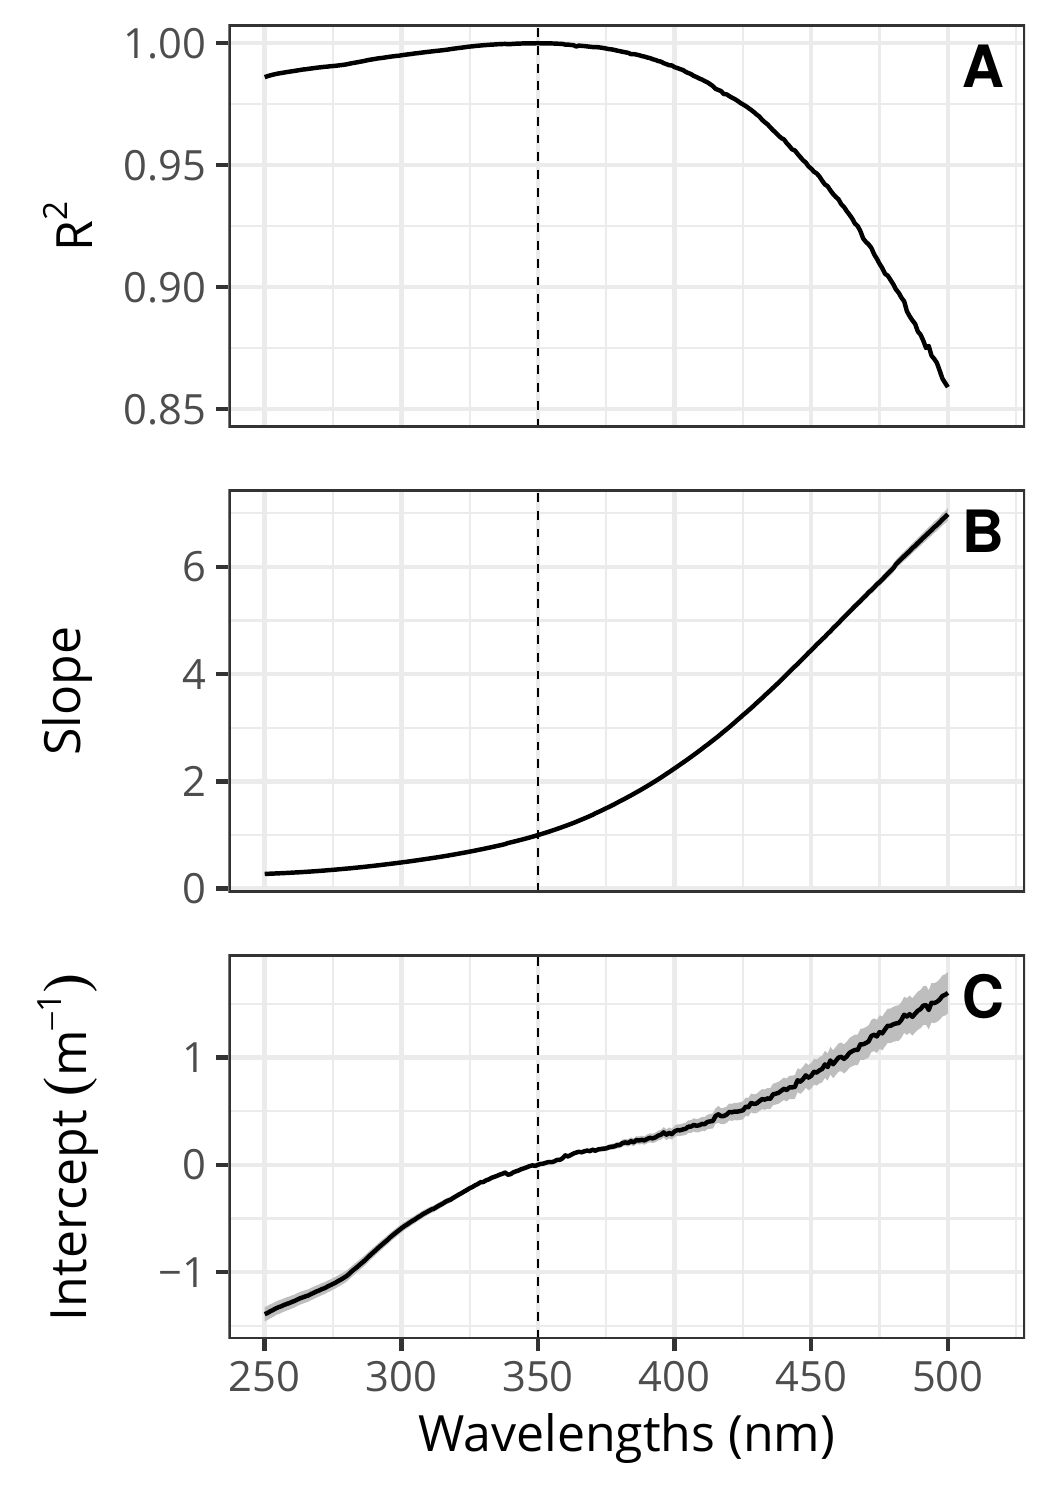
\includegraphics[scale = 1.5]{../../graphs/appendix2a}
	\caption{\label{first}Results of the linear regressions between a\textsubscript{CDOM}(350) and a\textsubscript{CDOM}($\lambda$). (\textbf{A}) Determination coefficients ($R^2$), (\textbf{B}) slopes and (\textbf{C}) intercepts of the linear regressions. Shaded areas (only visible in panel C) show the 95\% confidence interval of the estimated parameters. Panels contain the results of 251 linear models (one for each wavelength), each based on 2431 data points. Note that at $\lambda = 350$ nm (vertical dashed line), $R^2 = 1$, slope = 1 and intercept = 0. Note that for the Nelson et al. (2010) dataset (Table 1), absorption spectra were only available between 275 and 600 nm, and not included in this analysis.}
\end{figure}

\begin{figure}[h]
	\ContinuedFloat
	\centering
	\includegraphics[scale = 1]{../../graphs/appendix2b}
	\caption{\label{second}Heat map showing the determination coefficients ($R^2$) of the linear regressions between absorption values for each pair of wavelengths between 250 and 500 nm ($n = 63001, 0.83 \le R^2 \le 1$). Each regression is based on 2431 observations. Note that the diagonal of the plot shows $R^2 = 1$. }
\end{figure}

\clearpage
\newpage

\section*{Supplementary section 3}
\subsection*{Log-linear relationship between \boldmath{$a_{\text{CDOM}}(350)$} and DOC divided by ecosystems.}

\begin{figure}[h]
	\centering
	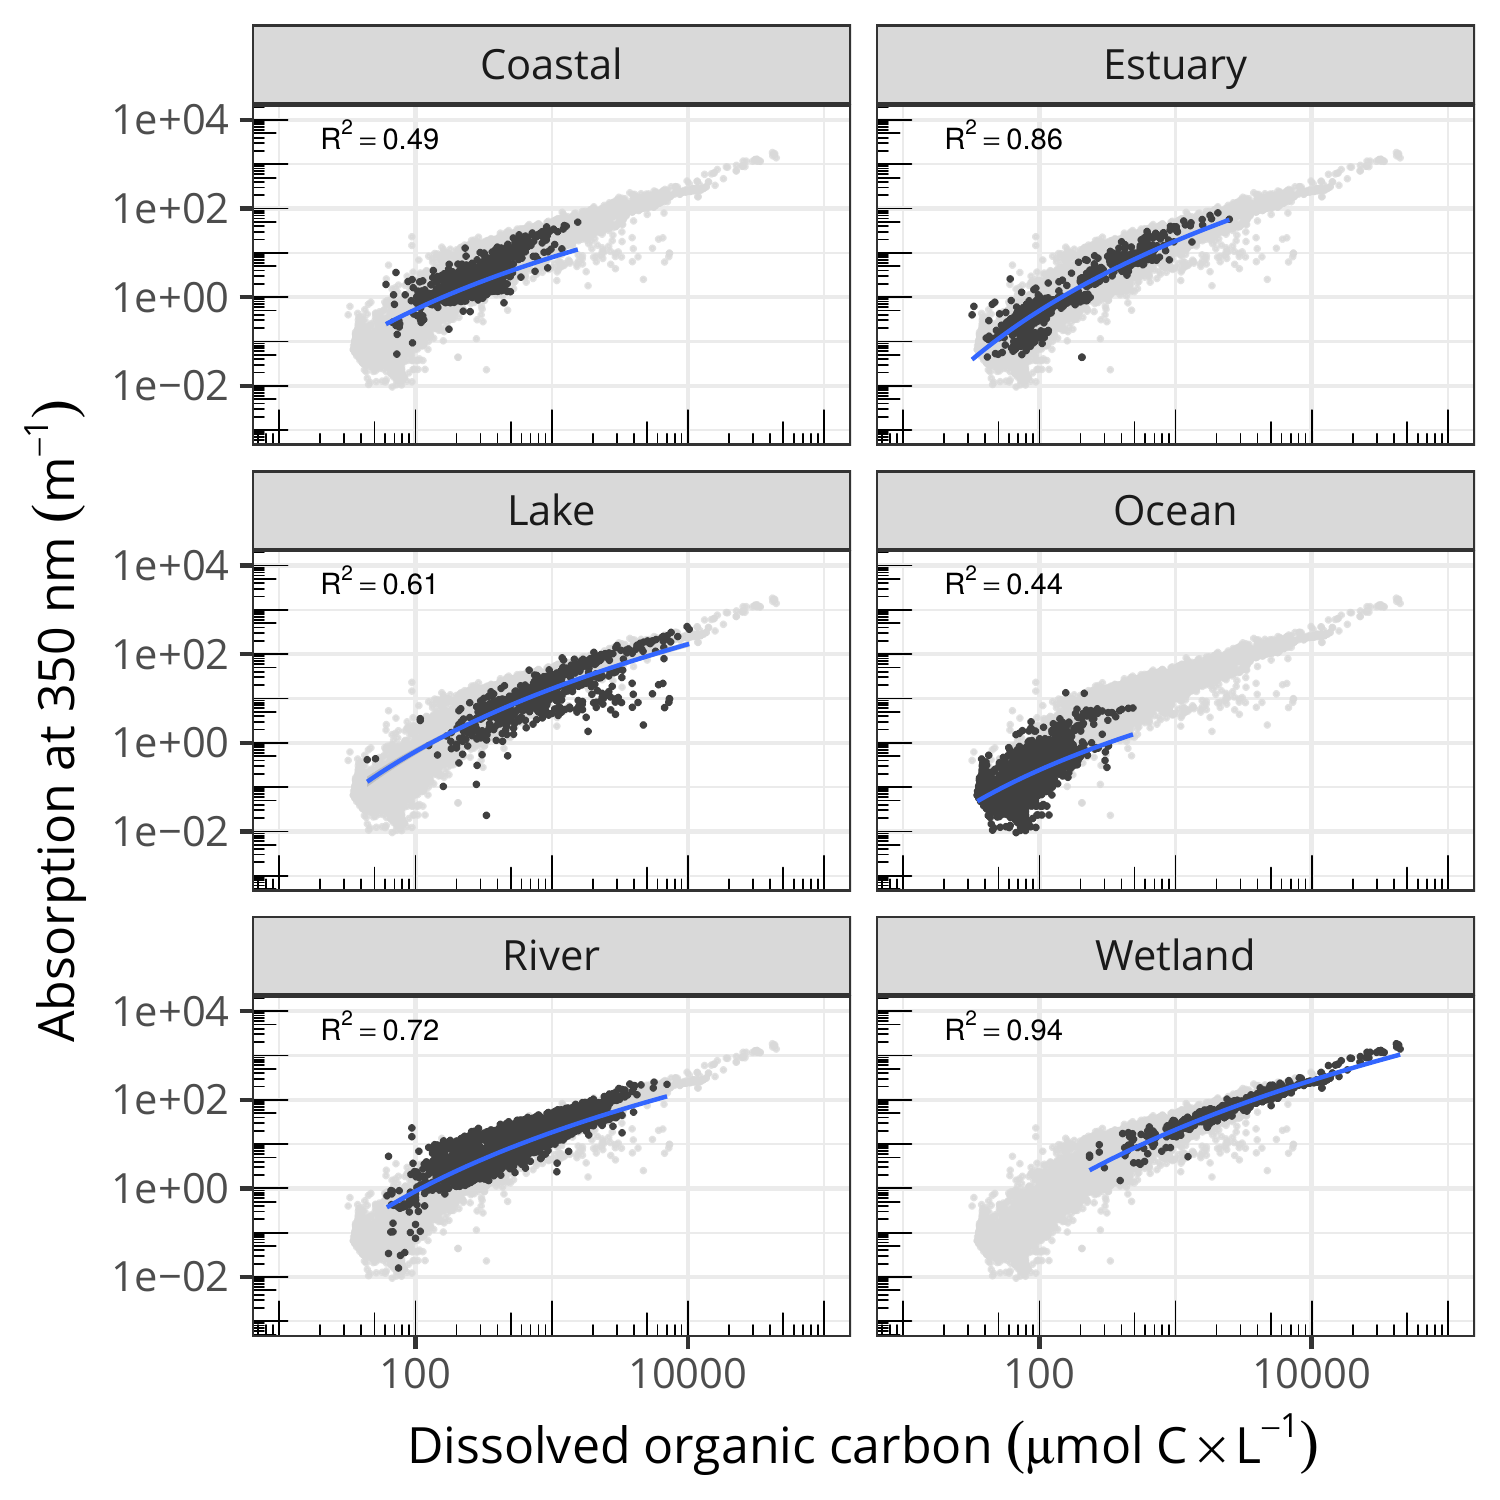
\includegraphics[scale = 1]{../../graphs/appendix3}

	\caption{The blue line is the fitted values of a linear model $y = \log(x)$. The shaded areas represent the 95\% confidence intervals. A total of 12808 observations are distributed across all panels (light gray dots in the background show the same global relation presented in Fig. 5).}
\end{figure}

\clearpage
\newpage

\section*{Supplementary section 4}
\subsection*{Residuals analysis}

\begin{figure}[H]
	\centering
	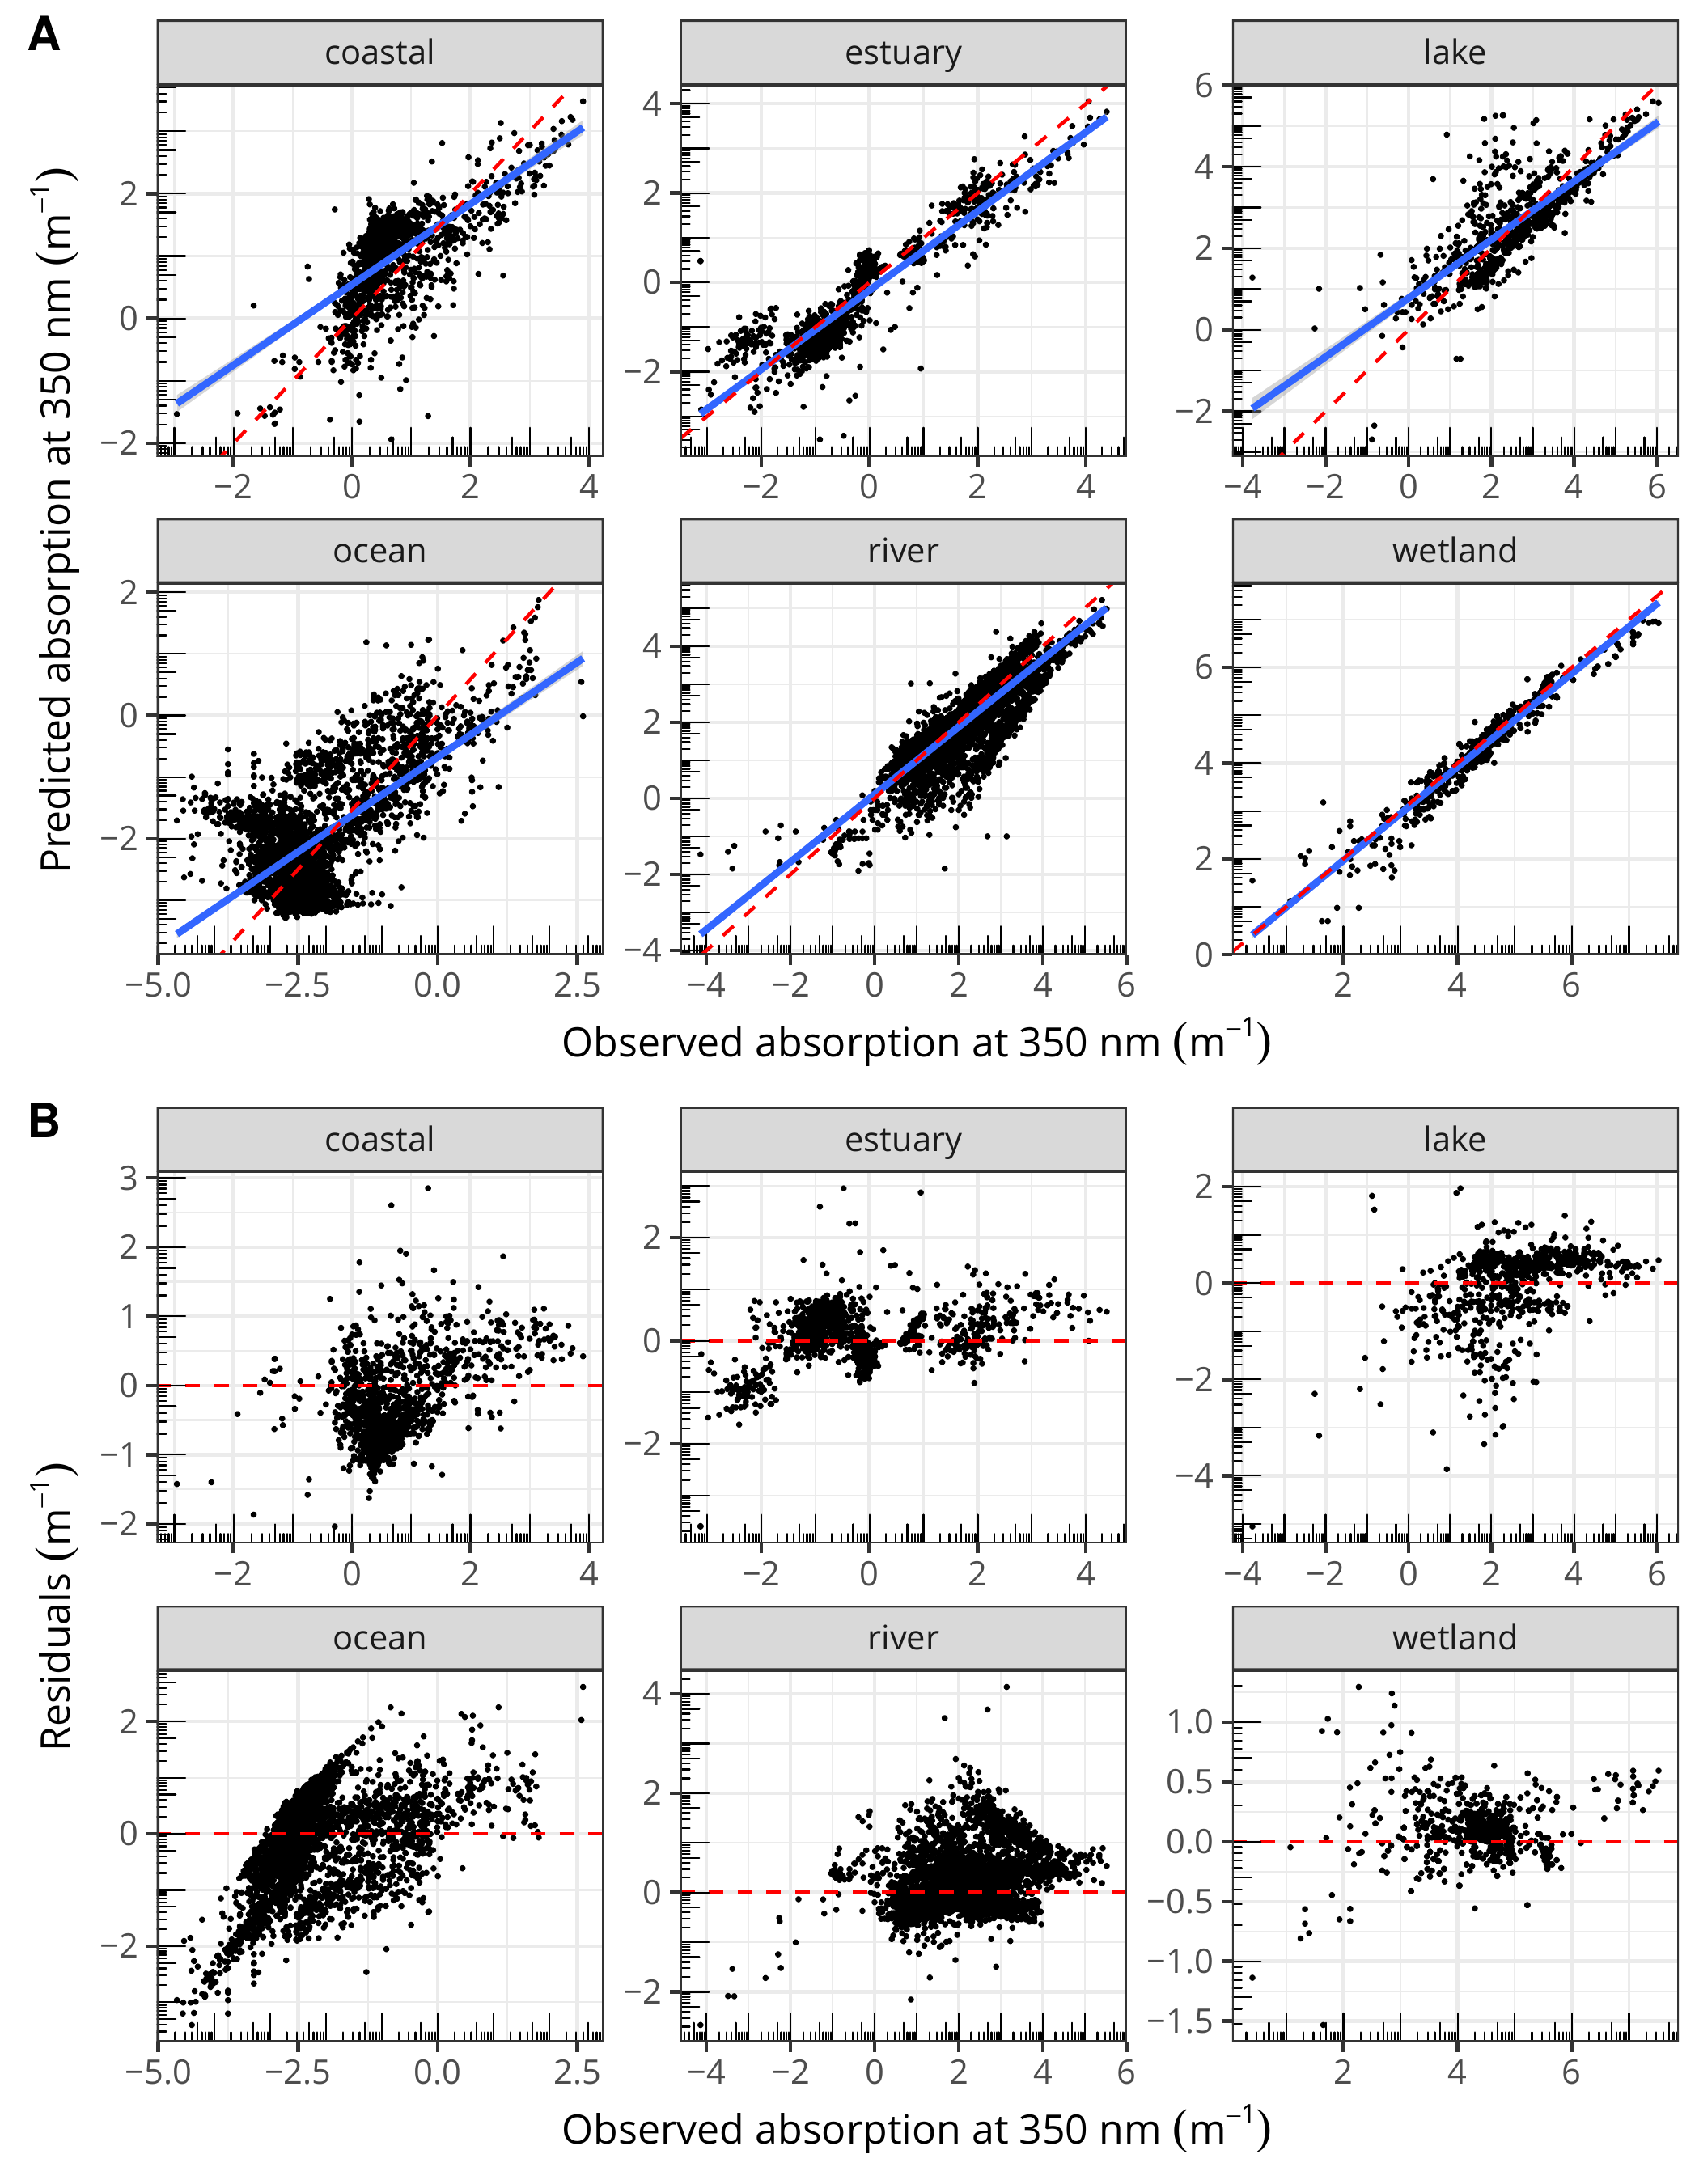
\includegraphics[scale = 0.8]{../../graphs/appendix4}
	\caption{\textbf{A} Scatterplots showing the relationship between observed and predicted values of $a_{\text{CDOM}}(350)$ (see Fig. 4). \textbf{B} Associated residual plots.}
\end{figure}

\clearpage
\newpage

\section*{Supplementary section 5}
\subsection*{Temporal and spatial distribution of the data}

\begin{figure}[h]
	\centering
	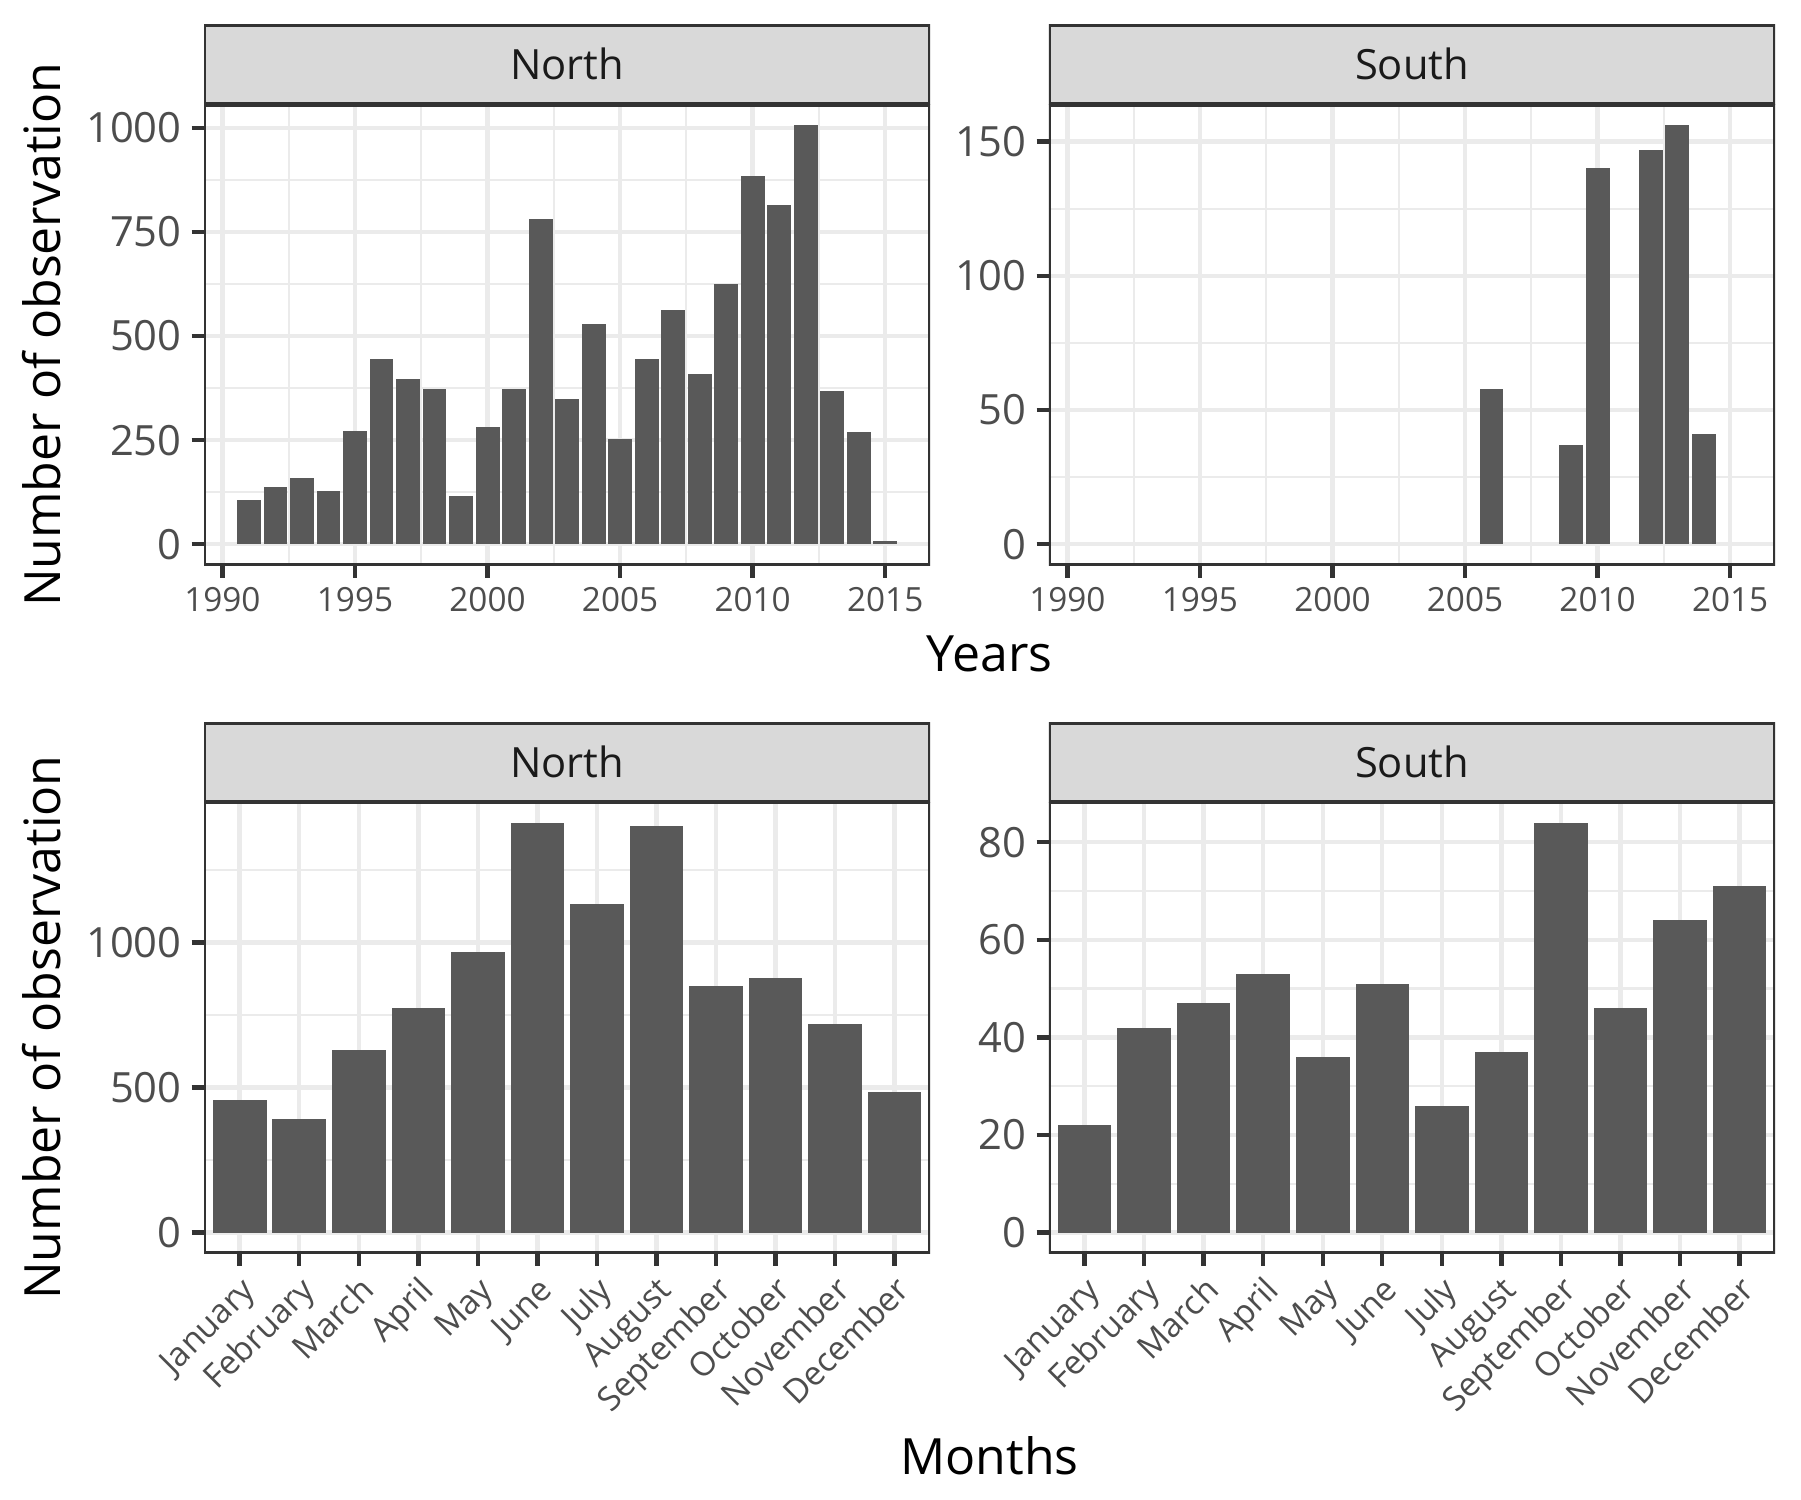
\includegraphics[scale = 1]{../../graphs/appendix5}
	\caption{Barplots showing how the data is distributed temporally across North and South hemisphere ($n = 12808$).}
\end{figure}

\end{document}
